%Wir verwenden eine DIN-A4-Seite und die Schriftgröße 12.
\documentclass[a4paper,12pt]{scrartcl} 


%Diese drei Pakete benötigen wir für die Umlaute, Deutsche Silbentrennung etc.
%Apple-Nutzer sollten anstelle von \usepackage[latin1]{inputenc} das Paket \usepackage[applemac]{inputenc} verwenden
%% \usepackage[latin1]{inputenc}
%%apt-get install texlive-lang-german kile kile-l10n  aspell-de 
%%damit ngerman keine Probleme mehr macht !!
\usepackage[utf8]{inputenc} 
\usepackage[T1]{fontenc}
\usepackage[ngerman]{babel}

%Das Paket erzeugt ein anklickbares Verzeichnis in der PDF-Datei.
%\usepackage{hyperref}

%Das Paket wird für die anderthalb-zeiligen Zeilenabstand benötigt
\usepackage{setspace}

%%HTWM-Vorlage - benoetigt apt-get install texlive-fonts-extra
\setcounter{tocdepth}{3}				%Schatelungstiefe Inhaltsverz.
\usepackage[utf8]{inputenc}			%deutsche Umlaute
\usepackage{german, ngerman}
\usepackage[ngerman]{babel}			%Rechtschreibprüfung
\usepackage{color,listings} 			%Quellcode Highlighting, bindet das
\usepackage{float}					%% GRAFIKPOSITION MITTELS [H] ERWZINGEN
%Paket Listings ein
\usepackage{listings}
\usepackage{color}
\usepackage{textcomp}
\usepackage[T1]{fontenc}				%srccode
\usepackage[scaled]{beramono}		%srccode
\usepackage{longtable}				%mehrseitige tabellen
\usepackage[tableposition=b]{caption}
\usepackage[pdftex, pdftoolbar=false, hyperfootnotes=false, bookmarks,
bookmarksopen, bookmarksnumbered, bookmarksopenlevel=2, pdfpagelabels=true,
pdfstartpage=3, pdfstartview=FitH,]{hyperref} %Verlinkungen
\usepackage{array}					%farbige Tabellen
\usepackage[table]{xcolor} 			%farbige Tabellen
\usepackage{graphicx}				% \includegraphics bnoetigt dies

\usepackage{fancyhdr, graphicx}		%% Logo auf Titelseite
\renewcommand{\headrulewidth}{0pt}
\fancyhead[L]{}
\fancyhead[R]{
  
\includegraphics[width=52mm]{./images/htwk.png}
}
%\usepackage{draftwatermark}			% wasserzeichen
	%Quelle: http://choorucode.com/2010/05/05/latex-adding-draft-watermark/?like=1&source=post_flair&_wpnonce=1c9f85538d
%\SetWatermarkText{VORABVERSION}		% wasserzeichen-text
%\SetWatermarkLightness{0.9}			% wasserzeichen-kontrast
%\SetWatermarkScale{2.5}				% wasserzeichen-zeichengroe\ss{}e

%%%% mathemathische Formeln zentrieren und vom Text absetzen mittels \[ E = mc^2 \] anstatt $ E = mc^2 $ %%%%
\usepackage{amsmath}
\usepackage{amsthm}
\usepackage{amsbsy}
\usepackage{amssymb}
%%%%%%%%%%%%%%%%%%%%%%%%%%%%%%%%%%%%%%%%%%%%%%%%%%%%%%%%%%%%%%%

\definecolor{Navy}{rgb}{0,0,0.5}
\definecolor{Gray}{gray}{0.5}
\definecolor{dunkelgrau}{rgb}{0.8,0.8,0.8}
\definecolor{hellgrau}{rgb}{0.95,0.95,0.95}
\definecolor{hellgrau2}{rgb}{0.93,0.93,0.93}

\hypersetup{
	colorlinks=true, 			% false: boxed links; true: colored links
	linkcolor=Navy,          		% color of internal links
	citecolor=Gray,        			% color of links to bibliography
	filecolor=magenta,      		% color of file links
	urlcolor=blue,           			% color of external links
	linkbordercolor={1 1 1}, 		% set to white
	citebordercolor={1 1 1} 		% set to white
}


%Einrückung eines neuen Absatzes
\setlength{\parindent}{0em}

%Definition der Ränder
\usepackage[paper=a4paper,left=30mm,right=30mm,top=30mm,bottom=30mm]{geometry}

%Abstand der Fussnoten
\deffootnote{1em}{1em}{\textsuperscript{\thefootnotemark\ }}

%Regeln, bis zu welcher Tiefe (section,subsection,subsubsection) Überschriften angezeigt werden sollen (Anzeige der Überschriften im Verzeichnis / Anzeige der Nummerierung)
%\setcounter{tocdepth}{3}
%\setcounter{secnumdepth}{3}

\fancypagestyle{htwkheader}
{
   \fancyhf{}	% clear all header and footer fields
  \fancyhead[RO]{
	\makebox[\textwidth]{	%% schiebe Logo nach aussen auf den Rand
		\rule{1				%% nach aussen schieben hoeherer Wert -> Logo weiter nach aussen
		  \textwidth}{0cm} %% nicht nach unten schieben = 0cm
			\includegraphics*[width=52mm]{./images/htwk.png}	%%Logo HTWK
	  }
  }
}



\begin{document}
 
%Beginn der Titelseite
\begin{titlepage}
\begin{small}
\vfill {HTWK Leipzig\\
Fachbereich IMN \\
Wintersemester 2013/2014}
\end{small}
 
\begin{center}
\begin{Large}
\vfill {\textsf{\textbf{
Die Internet Protokolle in Version 4 und 6\\
im Vergleich - ein \"Uberblick\\
}}}
\end{Large}
Beleg im Fach Hochgeschwindigkeitsnetze bei  Prof. Dr. Klaus Hänßgen
\end{center}
 
\begin{small}

\vfill
Marcel Kirbst, B.Sc. \\ Sieglitz 39 \\ 06618 Molauer Land \\
marcel.kirbst@htwk-leipzig.de\\
\today
\end{small}
 
\end{titlepage}
%Ende der Titelseite
 
%Inhaltsverzeichnis (aktualisiert sich erst nach dem zweiten Setzen)
\tableofcontents
\thispagestyle{empty}
 
%Beginn einer neuen Seite
\clearpage
 
%Anderthalbzeiliger Zeilenabstand ab hier
\onehalfspacing
 
\pagestyle{plain}
 
\section{Einleitung}
Dieser Beleg befasst sich mit der Vorstellung der Protokollfamilie IPv6. Neben einem kompakten Überblick über IPv6 soll auf die Notwendigkeit sowie die Vorzüge von IPv6 im Vergleich zu IPv4, der derzeit weltweit am meisten im Internet genutzten Protokollfamilie, eingegangen werden.\\
\\

Auch wenn klar sein muss, dass es im Umfang eines solchen Beleges nicht ann\"ahrend abschlie{\ss}end m\"oglich ist das Thema IPv6 ersch\"opfend vorzustellen, so hofft der Autor dem geneigten Leser doch einen \"Uberblick \"uber die Funktionen und Vorteile von IPv6 bieten zu k\"onnen.

\clearpage
\section{Warum IPv6 ?}
Das Internet ist heute überall im täglichen Leben präsent und wird von der UN inzwischen zu den Menschenrechten gezählt.\cite{uninet} Die im Internet heute noch am häufigsten verwendete Protokollfamilie ist IPv4. Wie der folgende Abschnitt darlegt, ist die weitere Verwendung von IPv4 aber mit immer mehr Problemen behaftet.

\subsection{Probleme mit IPv4}
Zu Beginn der Entwicklung des Internets war nicht abzusehen wie rasant und erfolgreich sich diese vollziehen würde. Ziel war einige wenige Rechnersysteme mit einander zu verbinden. Daher schien es beispielsweise mehr als ausreichend einen 32 Bit breiten Adressraum zu wählen, der somit $2^{32} = 4.294.967.296$ eindeutige Netzwerkadressen zulässt. In den 1970er Jahren entsprach das immerhin annährend einer IPv4-Adresse pro Erdenbewohner f\"ur eine geplante Vernetzung einiger weniger milit\"arisch genutzter Rechnersysteme.

\subsubsection{Adressknappheit}
Sp\"ater begannen auch Bildungseinrichtungen und nichtmilit\"arische Konzerne das Internet zu nutzen.
Zu dieser Zeit wurde IPv4 Adressraum relativ gro\ss{}z\"ugig verteilt. Viele Unternehmen und Bildungseinrichtungen der damaligen Zeit erhielten 24 Bit gro\ss{}e Adressbl\"ocke. Das bedeutet, dass dem jeweilgen Unternehmen ein Adressblock zugeteilt wurde, welcher $2^{24}$ also $16.777.216$ IPv4 Adressen umfasst. Beispiele f\"ur solche Unternehmen sind IBM (Adressraum 9.*.*.*), Hewlett-Packard (15.*.*.*) und Apple (17.*.*.*). Eine vollst\"andige Liste l\"asst sich unter \cite{ianaipv4list} einsehen.\\
\\
Beg\"unstigt wurde diese Problematik durch die anf\"angliche strikte Adresseinteilung in Klassen (Class A - E Netze), wobei es sich bei Class-A Netzen um besagte Netze mit 8 Bit langem Netzpr\"afix handelt. Class-B Netze besitzen ein Netzpr\"afix von 16 Bit und Class-C Netze einen Netzpr\"afix von 24 Bit. Es konnten somit nur Netzbl\"ocke f\"ur $2^{32} - 2^{24} = 256$ oder weniger Teilnehmer (Class-C Netze), $2^{32} - 2^{16} = 65.536$ oder weniger Teilnehmer (Class-B Netze) oder besagte $2^{32} - 2^{8} = 16.777.216$ zugeteilt werden. Beispielsweise bedeutete das f\"ur jede Einrichtung, die wenig mehr als 256 IPv4-Adressen ben\"otigte, ein Class-B Adressblock zu beantragen, auch wenn dann ein Gro\ss{}teil der Adressen ungenutzt blieb.\\
\\
Die nachtr\"agliche Einf\"uhrung einer Technik namens "`Classless Interdomain Routing"' (Abk\"urzung: CIDR) milderte die Problemstellung in der Weise ab, dass eine so genannte Netzwerkmaske zu jeder IPv4-Adresse angegeben wird, die angibt wieviele Bits der IPv4-Adresse den Netzwerkpr\"afix zugeordnet werden. Die Netzwerkmaske $255.255.0.0$ f\"ur die IPv4-Adresse $192.168.12.34$ definiert das Netzwerkpr\"afix $192.168$ sowie die Teilnehmeradresse $12.34$. Als Kurzschreibweise hat sich alternativ folgende Form verbreitet: 192.168.12.34/16. Hier gibt die Zahl nach dem Schr\"agstrich die Bitanzahl der Netzmaske an.\\
\\
Au\ss{}erdem ist zu erw\"ahnen, dass sich die IPv4-Adressen in einem Netzwerksegment nicht vollst\"andig Teilnehmern zuordnen lassen, da bestimmte Adressen wie beispielsweise $192.168.12.0/24$ (Bezeichner f\"ur dieses Netzsegment) oder $192.168.12.255/24$ (Broadcastadresse in diesem Netzsegment) eine besondere Bedeutung haben. \\
\\
Ein weiterer Umstand der die Problematik versch\"arft ist, dass die Zuteilung von IPv4-Adressbl\"ocken durch die IANA endg\"ultig ist. Eine M\"oglichkeit IPv4-Adressen zur\"uck zugewinnen ist nicht vorgesehen. 


\subsubsection{Konfiguration von Netzwerkger\"aten  unter Verwendung von IPv4}

Anf\"anglich musste jedes neue Netzwerkger\"at von Hand durch den Benutzer konfiguriert werden um im Netzwerk kommunizieren zu k\"onnen. Das umfasst mindestens die Vergabe einer IPv4-Adresse mit der zugeh\"origen Netzmaske. Soll das Ger\"at au\ss{}erdem noch mit dem Internet kommunizieren k\"onnen, ist die Angabe der IPv4-Adresse des Routers in diesem Netz sowie mindestens eines Domain Name Service-Servers (Abk\"urzung: DNS-Server) erforderlich.\\
\\
Um unerfahrenen, beziehungsweise unachtsamen Benutzern diese potentielle Fehlerquelle zu ersparen, wurde eine Technik namens Dynamic Host Configuration Protocol (Abk\"urzung: DHCP) \cite[RFC2131]{RFC2131} spezifiziert, die es erm\"oglicht die Konfiguration eines Netzwerkg\"er\"ates ohne Eingriff des Benutzers, nur durch einen DHCP-Server, welcher zustandsbasiert arbeitet,  in diesem Netzwerksegment vorzunehmen. Leider arbeitet auch dieser Mechanismus nicht immer zuverl\"assig und fehlerfrei. Beispielsweise ist es f\"ur ein Netzwerkger\"at durchaus m\"oglich manuell eine IPv4-Adresse zu konfigurieren und zu verwenden, die innerhalb des IPv4-Adresskontingentes liegt, der einem DHCP-Server zur Zuteilung an anfragende DHCP-Klienten zugeteilt wurde. Solche Adresskonflikte f\"uhren in der Regel zu Netzwerkproblemen.


\subsection{NAT}
Network Adress Translation (Abk\"urzung: NAT) \cite[RFC1631]{RFC1631} ist eine weitere Technik, die entwickelt wurde um die Adressknappheit in IPv4 abzumildern. In den meisten F\"allen ist ein Netzwerkger\"at nicht direkt mit dem Internet verbunden, sondern nur Teilnehmer in einem Netzwerk. In den meisten Netzwerken werden so genannte "`private IPv4-Adressen"' genutzt um die Netzwerkger\"ate zu adressieren. Das sind IPv4-Adressen die von der IANA speziell f\"ur diesen Zweck spezifiziert wurden und aus diesem Grund auch nicht im Internet genutzt werden k\"onnen. Router im Internet verwerfen Pakete, die als Sender- oder Empf\"angeradresse eine solche private IPv4-Adresse enthalten. Private IPv4-Adressen sind alle IPv4-Adressen aus den Bl\"ocken $10.0.0.0/8$ bis $10.255.255.255/8$, $172.16.0.0/12$ bis $172.31.255.255/12$ sowie $192.168.0.0/16$ bis $192.168.255.255/16$. \\
\\
Die Funktion eines Routers der NAT implementiert ist prinzipiell, dass alle Pakete von Netzwerkteilnehmen mit privater IPV4-Adresse im lokelen Netzwerk, die ins Internet geroutet werden sollen, vom Router so umgeschrieben werden, dass die private Absender-IP jedes Paketes durch die \"offentliche IP-Adresse des Routers ersetzt wird. Erh\"alt der Router Antwortpakete aus dem Internet die an diesen adressiert sind, schreibt er die Empf\"anger-IP wieder auf die private IP-Adresse des Netzwerkger\"ates um un leitet es dann weiter. Die Abbildung \ref{stdinetv4} am Ende des Kapitels soll dies illustrieren.\\

\begin{figure}[htb]
\begin{center}
 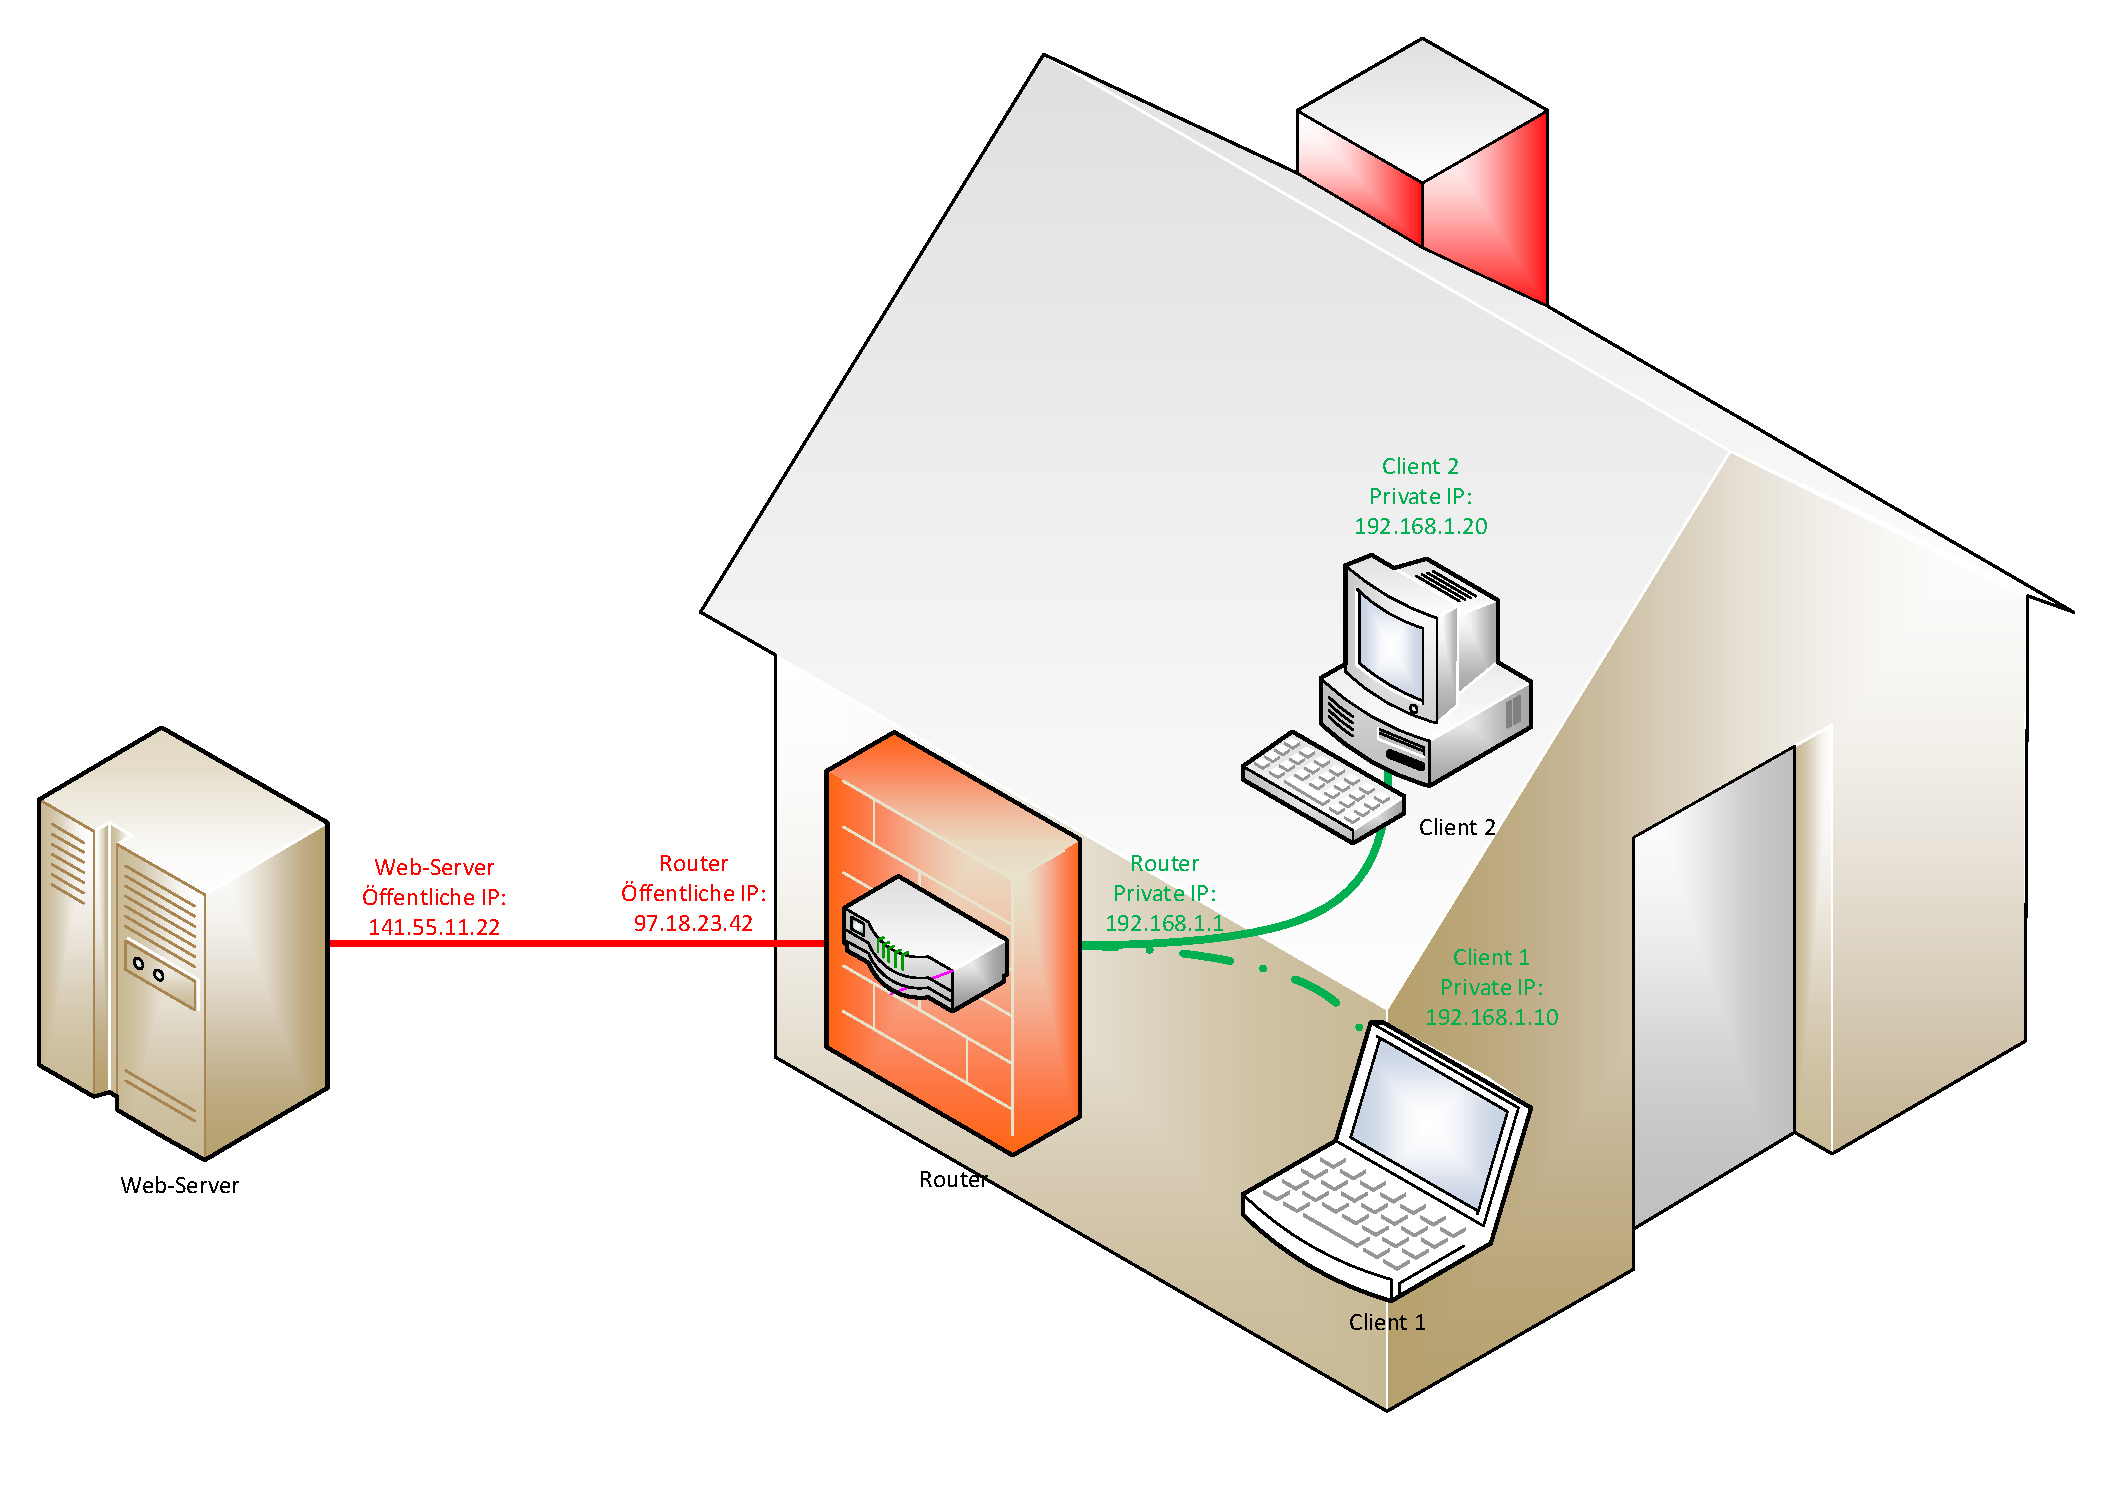
\includegraphics[width=1\hsize]{./Zeichnungen/IPv4NAT.pdf}
 \end{center}
\caption[Beispielhafte Standardkonfiguration eines Internetanschluss mit NAT, Quelle: Autor, verwendete Symbole unterliegen der
GPL]{\label{stdinetv4}Beispielhafte Standardkonfiguration eines Internetanschluss.}
\end{figure}

In einigen Szenarien, in denen weniger komplexe, verbindungsorientierte Protokolle wie beispielsweise HTTP eingesetzt werden funktioniert NAT einigerma\ss{}en zufriedenstellend. In komplexeren Protokollen wie dem File Transfer Protokoll (Abk\"urzung: FTP) oder dem Session Initiaton Protokoll (Abk\"urzung: SIP), in denen zum Beispiel im Laufe der Etablierung der Kommunikation weitere Ports f\"ur die Kommunikation zwischen den Endger\"aten ausgehandelt werden m\"ussen, st\"o{\ss}t NAT aber schnell an seine Grenzen, mit der Folge das diese Protokolle sich dann nicht oder zumindest nicht zufriedenstellend einsetzen lassen.\\
\\
Zwar kann dem zum Beispiel teilweise durch den Einsatz von spezifischen Proxy-Diensten auf dem Router f\"ur jedes einzelne Protokoll entgegen gewirkt werden, jedoch erh\"ot dieses Vorgehen die Komplexit\"at, den Verwaltungs- und Wartungsaufwand f\"ur die betreffenden Router.

\subsection{Ineffizienz in IPv4}
Einige Designentscheidungen bei der Entwicklung von IPv4 haben sich als ineffizient erwiesen. Beispielhaft sei hier die Verwendung einer Prüfsumme für den Paketheader genannt. Jedes mal wenn ein IPv4-Paket verändert wird muss die Prüfsumme des Paketheaders neu berechnet werden. Vor allem bei Netzwerkgeräten, die hohe Durchsätze an Datenmengen bewältigen sollen, beispielsweise die Core-Router von Internet Service Providern, sorgt das für Ressourcenengpässe beziehungsweise aufwändigere und damit teurere Hardware.\\
\\
Fixe Header der IPv4 Pakete sind unter mehreren Gesichtspunkten von Nachteil, da sie nicht nur die Flexibilität in der Verwendung des IPv4 Protokolls einschränken, sondern durch ihre fixe Größe auch eine Entlastung durch Weglassen nicht benötigter Teile des Paketheaders eine Steigerung der Effizienz verhindern.  \\
\\
Ein weiteres Effizienzproblem bei der Verwendung von IPv4 ist der im Laufe der Zeit stark angewachsene Umfang der Routingtabellen. Wünschenswert ist, dass der Umfang der Routingtabellen möglichst gering bleibt, um die Router im Internet so gut wie möglich zu entlasten. Durch die immer problematischere Adressknappheit im IPv4-Adressraum ist auch eine immer stärkere Segmentierung der IPv4-Adressen und IPv4-Adressbereiche zu beobachten mit der Konsequenz immer stärker anwachsender Routingtabellen in den Routern.\\



\clearpage
\section{\"Uberblick zu IPv6}
Nachdem im vorangegangenen Kapitel viele der Nachteile von IPv4 erwähnt wurden, sollen nun im Folgenden die wichtigsten Neuerungen von IPv6 vorgestellt werden. 

\subsection{Gr\"o{\ss}e  des Adressraums}

Offenkundigste Neuerung von IPv6 ist die Erweiterung des Adressraums auf 128 Bit. Mit einem 128 Bit breiten Adressraum lassen sich \\
$2^{128} = 340.282.366.920.938.463.463.374.607.431.768.211.456$ individuelle Adressen bilden. Vergleichweise gering fällt der 32 Bit breite IPv4-Adressraum aus, denn hier lassen sich "`nur"' $2^{32} = 4.294.967.296$ individuelle Adressen bilden. \\
\\
Bestand eine IPv4-Adresse aus vier durch einen Dezimalpunkt getrennten Ziffern mit Werten von jeweils zwischen 0 und 255, also zum Beispiel 85.114.130.113, musste für IPv6 mit seinen 128 Bit großen Adressen ein neues Konzept entwickelt werden.
Der Ziffernbereich umfasst jetzt den Bereich aller Hexadezimalziffern, also 0 bis 9 und A bis F. Bis zu vier Hexadezimalziffern werden zu einem Block zusammen gefasst, wobei führende Nullen nicht ausgeschrieben werden m\"ussen. Acht dieser Blöcke, welche durch Doppelpunkte von einander abgegrenzt werden, bilden eine gültige IPv6-Adresse, die vollständig ausgeschrieben  beispielsweise so aussehen kann:  \[ 2001:41d0:0001:f7bb:0000:0000:0000:0001 \]\\
\\
Um den Umgang mit IPv6-Adressen komfortabler zu gestalten, gibt es mehrere Möglichkeiten, IPv6 Adressen verkürzt darzustellen. So müssen, wie bereits erwähnt, führende Nullen innerhalb eines Block nicht zwingend angegeben werden. Weiterhin ist es pro IPv6-Adresse möglich einen Bereich aus Nullen, der sich über mehrere Blöcke erstrecken kann, wegzulassen und stattdessen nur die Doppelpunkte am Beginn und dem Ende dieses Null-Bereiches darzustellen. Es ist jedoch zu beachten das pro IPv6 Adresse jeweils immer nur ein Nullbereich weggelassen werden darf, da die IPv6 Adresse sonst nicht mehr eineindeutig ist. Durch Anwendung dieser Konventionen lässt sich die oben genannte, voll ausgeschrieben IPv6 Adresse
\[ 2001:41d0:0001:f7bb:0000:0000:0000:0001 \]
nun viel kürzer, jedoch trotzdem eineindeutig darstellen:
 \[ 2001:41d0:1:f7bb::1 \]
 

\subsection{mehrere IPv6-Adressen pro Netzwerkschnittstelle}

Ein Umstand, der in IPv4 oft zu Problemen f\"uhrte ist, dass pro aktiver Netzwerkschnittstelle nur eine IPv4-Adresse zugewiesen werden kann. Soll einem Netzwerkclient zum Beispiel dynamisch eine IPv4-Adresse zugewiesen werden, kann der Client mit dem Server (und umgekehrt) nur \"uber Broadcast-Adressen kommunizieren, bis der Client eine IPv4-Adresse zugewiesen bekommen hat.\\
\\
Ein fester und grundlegender Umstand vom IPv6 ist die Tatsache, dass jede Netzwerkschnittstelle mit mehreren IPv6-Adressen umgehen k\"onnen muss. Sobald eine Netzwerkschnittstelle in einem IPv6-f\"ahigem System den betriebsbereiten Zustand erreicht, ist ihr schon mindestens eine IPv6-Adresse zugewiesen. Dabei handelt es sich um die so genannte Link-Local-Adresse. Diese ist nur im lokalen Netzwerkkontext g\"ultig und wird unter anderem aus der MAC-Adresse der jeweiligen Netzwerkschnittstelle unter Zuhilfenahme von Zufallsalgorithmen gebildet. Mit der Link-Local-Adresse kann ein Netzwerkclient mit anderen lokalen Netzwerkteilnehmern kommunizieren sowie weitere Netzwerkparameter austauschen und aushandeln.

\subsection{Spezielle IPv6-Adressen}

Von den $2^{128}$ IPv6-Adressen sind laut \cite[RFC5156]{RFC5156} bestimmte Adressbereiche für besondere Aufgaben reserviert, von denen nachfolgend beispielhaft einige genannt seien. 

\begin{longtable}{p{24mm}>{
	\columncolor[gray]{0.97}}p{48mm}p{65mm}>{\columncolor[gray]{0.97}}p{33mm}}
	\rowcolor[gray]{.9}\textbf{Adressprefix} & \textbf{Bezeichnung laut IETF} & \textbf{Beschreibung} \\
		::1/128 & Node-Scoped Unicast - loopback address & Lokale Loopback-Adresse (\"ahnlich 127.0.0.1 in IPv4), sollten nicht im Internet auftauchen\\
		\rowcolor[gray]{.95} ::1/128 & Node-Scoped Unicast - unspecified address & bisher unpezifiziert (Stand RFC5156 von April 2008 )\\
		::FFFF:0:0/96 & IPv4 mapped adress & IPv4 gemappte Adressen. Adressen dieses Typs sollten im \"offentlichen Internet nicht auftauchen.\\
		\rowcolor[gray]{.95} ::<ipv4-address>/96 & IPv4-Compatible Addresses & Adressbereich um IPv4-Adressen für andere IPv6-Ger\"ate kompatibel einzubetten \\  
\caption{LautRFC 5161 vordefinierte Adressprefixe in IPv6}
\label{LautRFC 5161 vordefinierte Adressprefixe in IPv6}
\end{longtable}

\subsection{Automatische Netzwerkkonfiguration}
Bei Verwendung von IPv6 ist es den Netzwerkger\"aten m\"oglich, \"uber so genannte "'Neighbor Discovery Protocol"'  \cite[RFC3122]{RFC3122},  \cite[RFC4861]{RFC4861} zu erfragen, ob sich Router im gleichen Netzwerksegment befinden, wie die Netzwerkclients selbst. Dazu generiert ein Netzwerkger\"at das in einem IPv6-Netzwerk kommunizieren m\"ochte, zuerst eine so genannt "'Link Local Adresse"'. Diese Link-Local-Adresse generiert sich das Ger\"at selbst, unter anderem aus der MAC-Adresse der betreffenden Netzwerkschnittstelle. Charakteristisch f\"ur diese Link-Local-Adressen ist, dass diese immer mit dem Prefix $fe80::$ beginnen. Eine weitere Besonderheit ist der G\"ultigkeitsbereich von Link-Local-Adressen, diese sind nur im aktuellen Netzwerksegment g\"ultig und werden nicht geroutet. In der Konsequenz bedeutet das, dass ein Netzwerkger\"at \"uber die Link-Local-Adresse nur mit anderen Netzwerkger\"aten kommunizieren kann, die sich im gleichen Netzwerksegment befinden. In der folgenden Grafik ist eine beispielhafte IP-Konfiguration des Autors abgebildet, die f\"ur diesen Beleg erstellt wurde.

\begin{figure}[htb]
\begin{center}
 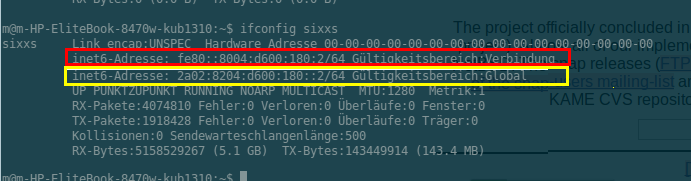
\includegraphics[width=1\hsize]{./images/ifconfig.png}
 \end{center}
\caption[IP-Konfiguration beispielhaft beim Autor, Quelle: Autor,]{\label{ifconfig}IP-Konfiguration beispielhaft beim Autor}
\end{figure}

F\"ur die Recherche zu diesem Beleg wurde auf einem Laptop die Linux-Distribution Kubuntu 12.04 LTS installiert. Der Aufruf des Befehls \textit{ifconfig} meldet f\"ur die Netzwerkschnittstelle "'sixxs"' (Anmerkung: sixxs.net ist ein Netzwerktunnel um Internetzug\"angen ohne natives IPv6 IPv6-Konnektivit\"at zu verschaffen, siehe dazu folgendes Kaptiel) zeigt rot umrahmt die Link-Local-Adresse $fe80::8004:d600:180:2/64$, die nur lokal g\"ultig ist, sowie die global g\"utige IPv6-Adresse $2a02:8204:d600:180::2$, in der Grafik gelb umrahmt.\\
\\
Nachdem sich ein Netzwerkger\"at eine Link-Lokal-Adresse zugewiesen hat, kann dieses, wie bereits oben erw\"ahnt, mit allen anderen Netzwerkger\"aten im gleichen Netzwerksegemnt kommunizieren, beispielsweise um so genannte Router-Advertisements abzusetzen. Das sind Netzwerkanfragen, auf die jeder IPv6-f\"ahige Router im Netzwerksegment antworten muss. Der Router kann dann in der Antwort dem anfragenden Netzwerkger\"at seine eigene IPv6-Adresse sowie das global g\"ultige IPv6-Prefix f\"ur dieses Netzwerksegment mitteilen. Wenn dies erfolgt ist, kann sich das anfragende Netzwerkger\"at aus dem globalen Prefix eine IPv6-Adresse mit globaler G\"ultigkeit generieren, mit deren Hilfe eine vollst\"andige Netzwerkkonnektivit\"at gegeben ist. 


\clearpage
\section{L\"osungsans\"atze in IPv6 zu den Problemen mit IPv4}
In diesem Kapitel sollen einige Vorz\"uge von IPv6 angef\"uhrt werden, die Probleme in IPv4 l\"osen.
 
\subsection{Beseitigung der Adressknappheit auf absehbare Zeit}
Durch den 128 Bit gro{\ss}en Adressraum und der damit verbundenen enormen Menge an zur Verf\"ugung stehenden Adressen sollten der Menschheit f\"ur die n\"achsten Jahrzehnte hinreichend viele IPv6-Adressen zur Verfügung stehen.  Um die enorme Dimension des Adressraums von IPv6 zu verdeutlichen, soll ein kurzes Rechenbeispiel dienen:\\
\\
Die Oberfläche der Erde umfasst grob geschätzt 510 Millionen Quadratkilometer, also $510.000.000.000.000.000.000 mm^2$ . Stellt man diese Fl\"ache der Anzahl der m\"oglichen IPv6-Adressen von $2^{128} = 340.282.366.920.938.463.463.374.607.431.768.211.456$ gegen\"ueber kommt man zu dem Ergebnis, das jedem Quadratmillimeter der Erdoberfl\"ache immernoch theoretisch $667.220.327.295.957.771 $ IPv6-Adressen zugewiesen werden k\"onnen. Praktisch betrachtet ist diese Zahl nicht ganz korrekt, da wie im voran gegangenen Kapitel beschrieben, bestimmte Adressen im IPv6-Adressraum reserviert sind. Dieser Vergleich soll dem Leser aber dennoch verdeutlichen das jedem Quadratmillimeter der Erdoberfl\"ache circa. 155 Millionen mal mehr IPv6-Adressen zugewiesen werden k\"onnen, als im gesamten IPv4-Adressraum (der ja nur 32 Bit gross) ist zur Verf\"ugung stehen. Die folgende Grafik soll den enormen Umfang an IPv6-Adressen im Vergleich zum Umfang der IPv4-Adressen f\"ur den Leser noch einmal illustrieren:

\clearpage

\begin{figure}[htb]
\begin{center}
 
\includegraphics[width=1\hsize]{./images/earth.png}
 \end{center}
\caption[Illustration: Mengenvergleich IPv4-Adressen f\"ur die gesamte Erdbev\"olkerung zu IPv6-Adressen pro Quadratmillimeter Erdoberfl\"ache. Quelle Illustration: Autor, Quelle Erdfoto: \url{http://upload.wikimedia.org/wikipedia/commons/6/6f/Earth_Eastern_Hemisphere.jpg}]{\label{earth}Illustration: Mengenvergleich IPv4-Adressen f\"ur die gesamte Erdbev\"olkerung zu IPv6-Adressen pro Quadratmillimeter Erdoberfl\"ache.  Quelle Illustration: Autor, Quelle Erdfoto: \url{http://upload.wikimedia.org/wikipedia/commons/6/6f/Earth_Eastern_Hemisphere.jpg}}
\end{figure}

\subsection{Vereinfachte Netzwerkwartung}

Unerfahrene Nutzer m\"ussen viel weniger administrativ t\"atig werden als in IPv4. Im Normalfall muss der Benutzer nichts weiter tun, als sein Ger\"at mit dem Netzwerk verbinden und einschalten. Somit sinkt auch die Fehlerquote durch Fehlkonfigurationen. Beispielsweise m\"ussen Router nicht mehr von Hand konfiguriert werden. In IPv6 existieren so genannte \textit{Router-Advertisements}. Wenn ein Netzwerkclient in einem IPv6-Netzwerk benachbarte Router anfragt, m\"ussen sich laut IPv6-Standard alle Router in diesem Netzwerk mit einem Router-Advertisement dem Netzwerkclient gegen\"uber bekannt machen. Dem Netzwerkger\"at stehen im Anschluss alle Informationen zur Verf\"ugung, die f\"ur eine vollst\"andige Internetkonnektivit\"at erforderlich sind. 

\subsection{Verkleinerung der Routingtabellen}
In den Standards zu IPv6 ist vorgesehen, dass jedem Kunden mindestens ein /64-Netz zugeteilt wird. Indem man Kunden komplette Netze zuteilt und die Adressverteilung dem Kunden, beziehungsweise dessen Router selbst überlässt, schrumpft der Umfang der Routingtabellen, die öffentliche Router im Internet vorhalten müssen, erheblich. Die folgende Grafik, die der Website unter \cite{ipv4v6map} entliehen ist, soll diesen Umstand visualisieren.

\begin{figure}[htb]
\begin{center}
 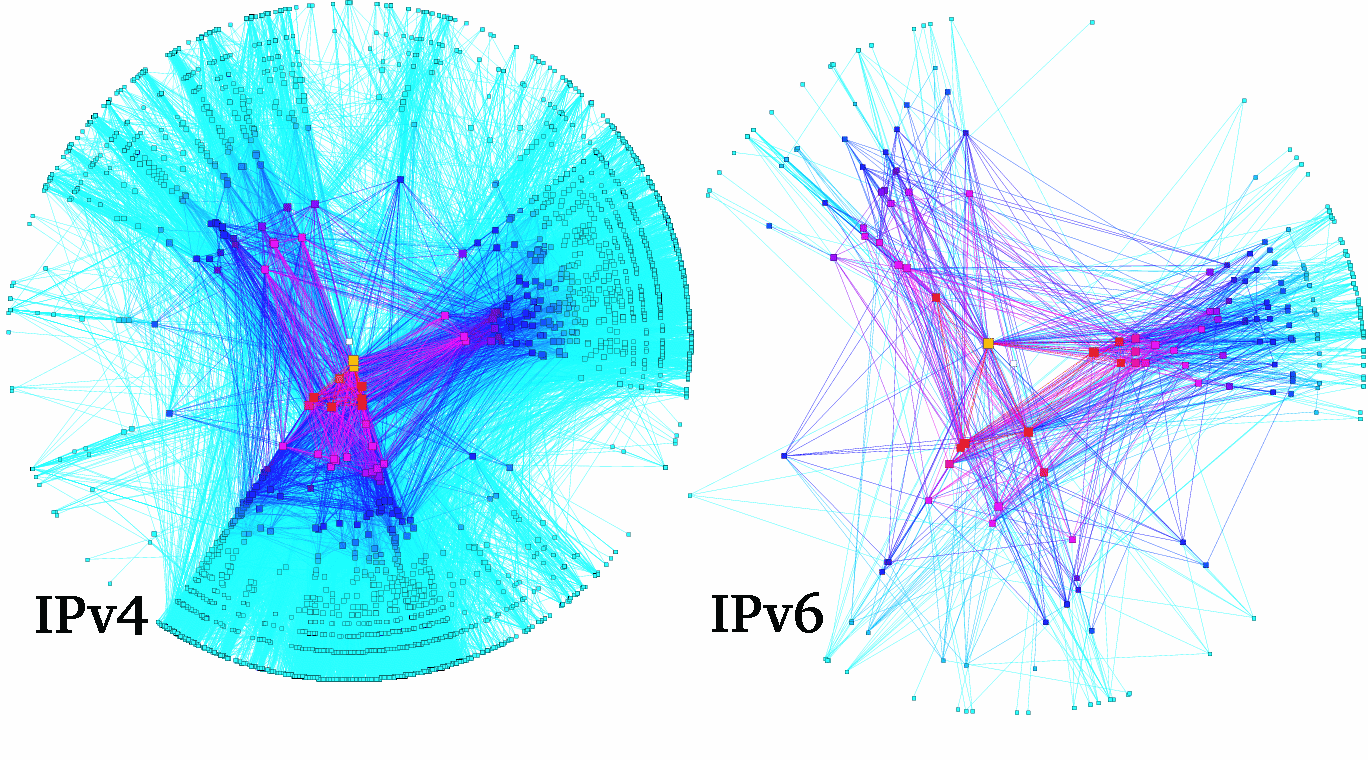
\includegraphics[width=.7\hsize]{./images/ipv4v6map.png}
 \end{center}
\caption[Visuelle Darstellung des Umfangs der Routingtabellen in IPv4 und IPv6, Quelle: \url{http://greenbyte.ch/wp-content/uploads/2012/08/ipv4-ipv6.gif?cf3116}]{\label{ipv4v6map}Visuelle Darstellung des Umfangs der Routingtabellen in IPv4 und IPv6, Quelle: \url{http://greenbyte.ch/wp-content/uploads/2012/08/ipv4-ipv6.gif?cf3116}}
\end{figure}

\clearpage
\subsection{Flexible Paketheader in IPv6}
 Bei der Verwendung von IPv6 existieren keine statischen Paketheader mehr, wie es bei der Verwendung von IPv4 der Fall ist. IPv6-Paketheader haben zwar eine fixe Grösse von 40 Byte, lassen sich je nach Bedarf flexibel durch so genannte "'Extensions Header"' erweitern. 
Ein Paketheader in IPv6 besteht aus den Feldern 
\begin{itemize}
	\item IP-Version (4 Bit)
	\item Traffic Class (8 Bit)
	\item Flow Label (20 Bit)
	\item Payload Length (16 Bit)
	\item \textbf{Next Header} (8 Bit)
	\item Hop Limit (8 Bit)
	\item Source Address (128 Bit)
	\item Destination Address (128 Bit). 
\end{itemize}

Die Gesamtgr\"o{\ss}e eines IPv6-Pakets betr\"agt also 320 Bit, was 40 Byte entspricht. Im Feld Next Header können dann gegebenenfalls Erweiterungsheader angegeben werden.  

Ein solcher Erweiterungsheader besteht dann aus den Feldern:
\begin{itemize}
 	\item Hop by Hop Options (variable Gr\"o{\ss}e)
	\item  Routing  (variable Gr\"o{\ss}e)
	\item Fragment (64 Bit)
	\item Authentication Header (variable Gr\"o{\ss}e)
	\item Encapsulating Security Payload  (variable Gr\"o{\ss}e)
	\item Destination Options  (variable Gr\"o{\ss}e)
	\item Mobility  (variable Gr\"o{\ss}e) und 
	\item No Next Header, welches das Ende des Erweiterungsheaders anzeigt. 
\end{itemize}

Somit ist sichergestellt, dass die IPv6-Header so klein wie möglich und so groß wie unbedingt nötig sind.  

\subsection{NAT in IPv6}
Wenn IPv6 den Vorgaben entsprechend betrieben wird, umfasst das unter anderem, dass jedem Teilnehmer im Internet von seinem Internet Service Provider ein 64 Bit gro{\ss}er  IPv6-Adressblock zugeteilt wird. Im Detail wird dem Kunden nur noch ein Adressprefix von 64 Bit zugeteilt. Wie der Kunde beziehungsweise dessen Netzwerkger\"ate die restlichen 64 Bit im lokalen Netzwerk verteilen, ist dem Kunden beziehungsweise dessen Netzwerkger\"aten  \"uberlassen. Ein gro{\ss}er Vorteil ist hierbei, dass jede einzelne IPv6-Adresse aus diesem 64 Bit gro{\ss}em Adressblock global routbar ist und somit nicht mehr die Notwenigkeit besteht Technologien wie NAT einsetzen zu m\"ussen, um nur lokal g\"ultige IPv4-Adressen auf eine einzelne, global g\"ultige IPv4-Adresse des Routers abzubilden.\\
\\

Ein Router, der im heimischen Netzwerk die Schnittstelle zum Internet darstellt, ist nun nicht mehr, wie bei IPv4, gezwungen die Netzwerkpakete f\"ur jedes Netzwerkger\"at im lokalen Netzwerk per NAT zu modifizieren. Da jedes Netzwerkger\"at bei Verwendung von IPv6 seine eigene global g\"ultige Adresse hat, ist eine eineindeutige Zuordnung der eingehenden und ausgehenden Netzwerkpakete zu den Netzwerkger\"aten f\"ur den Router ohne Probleme m\"oglich.  Folgende Grafik soll beispielhaft den Sachverhalt verdeutlichen:

\begin{figure}[htb]
\begin{center}
 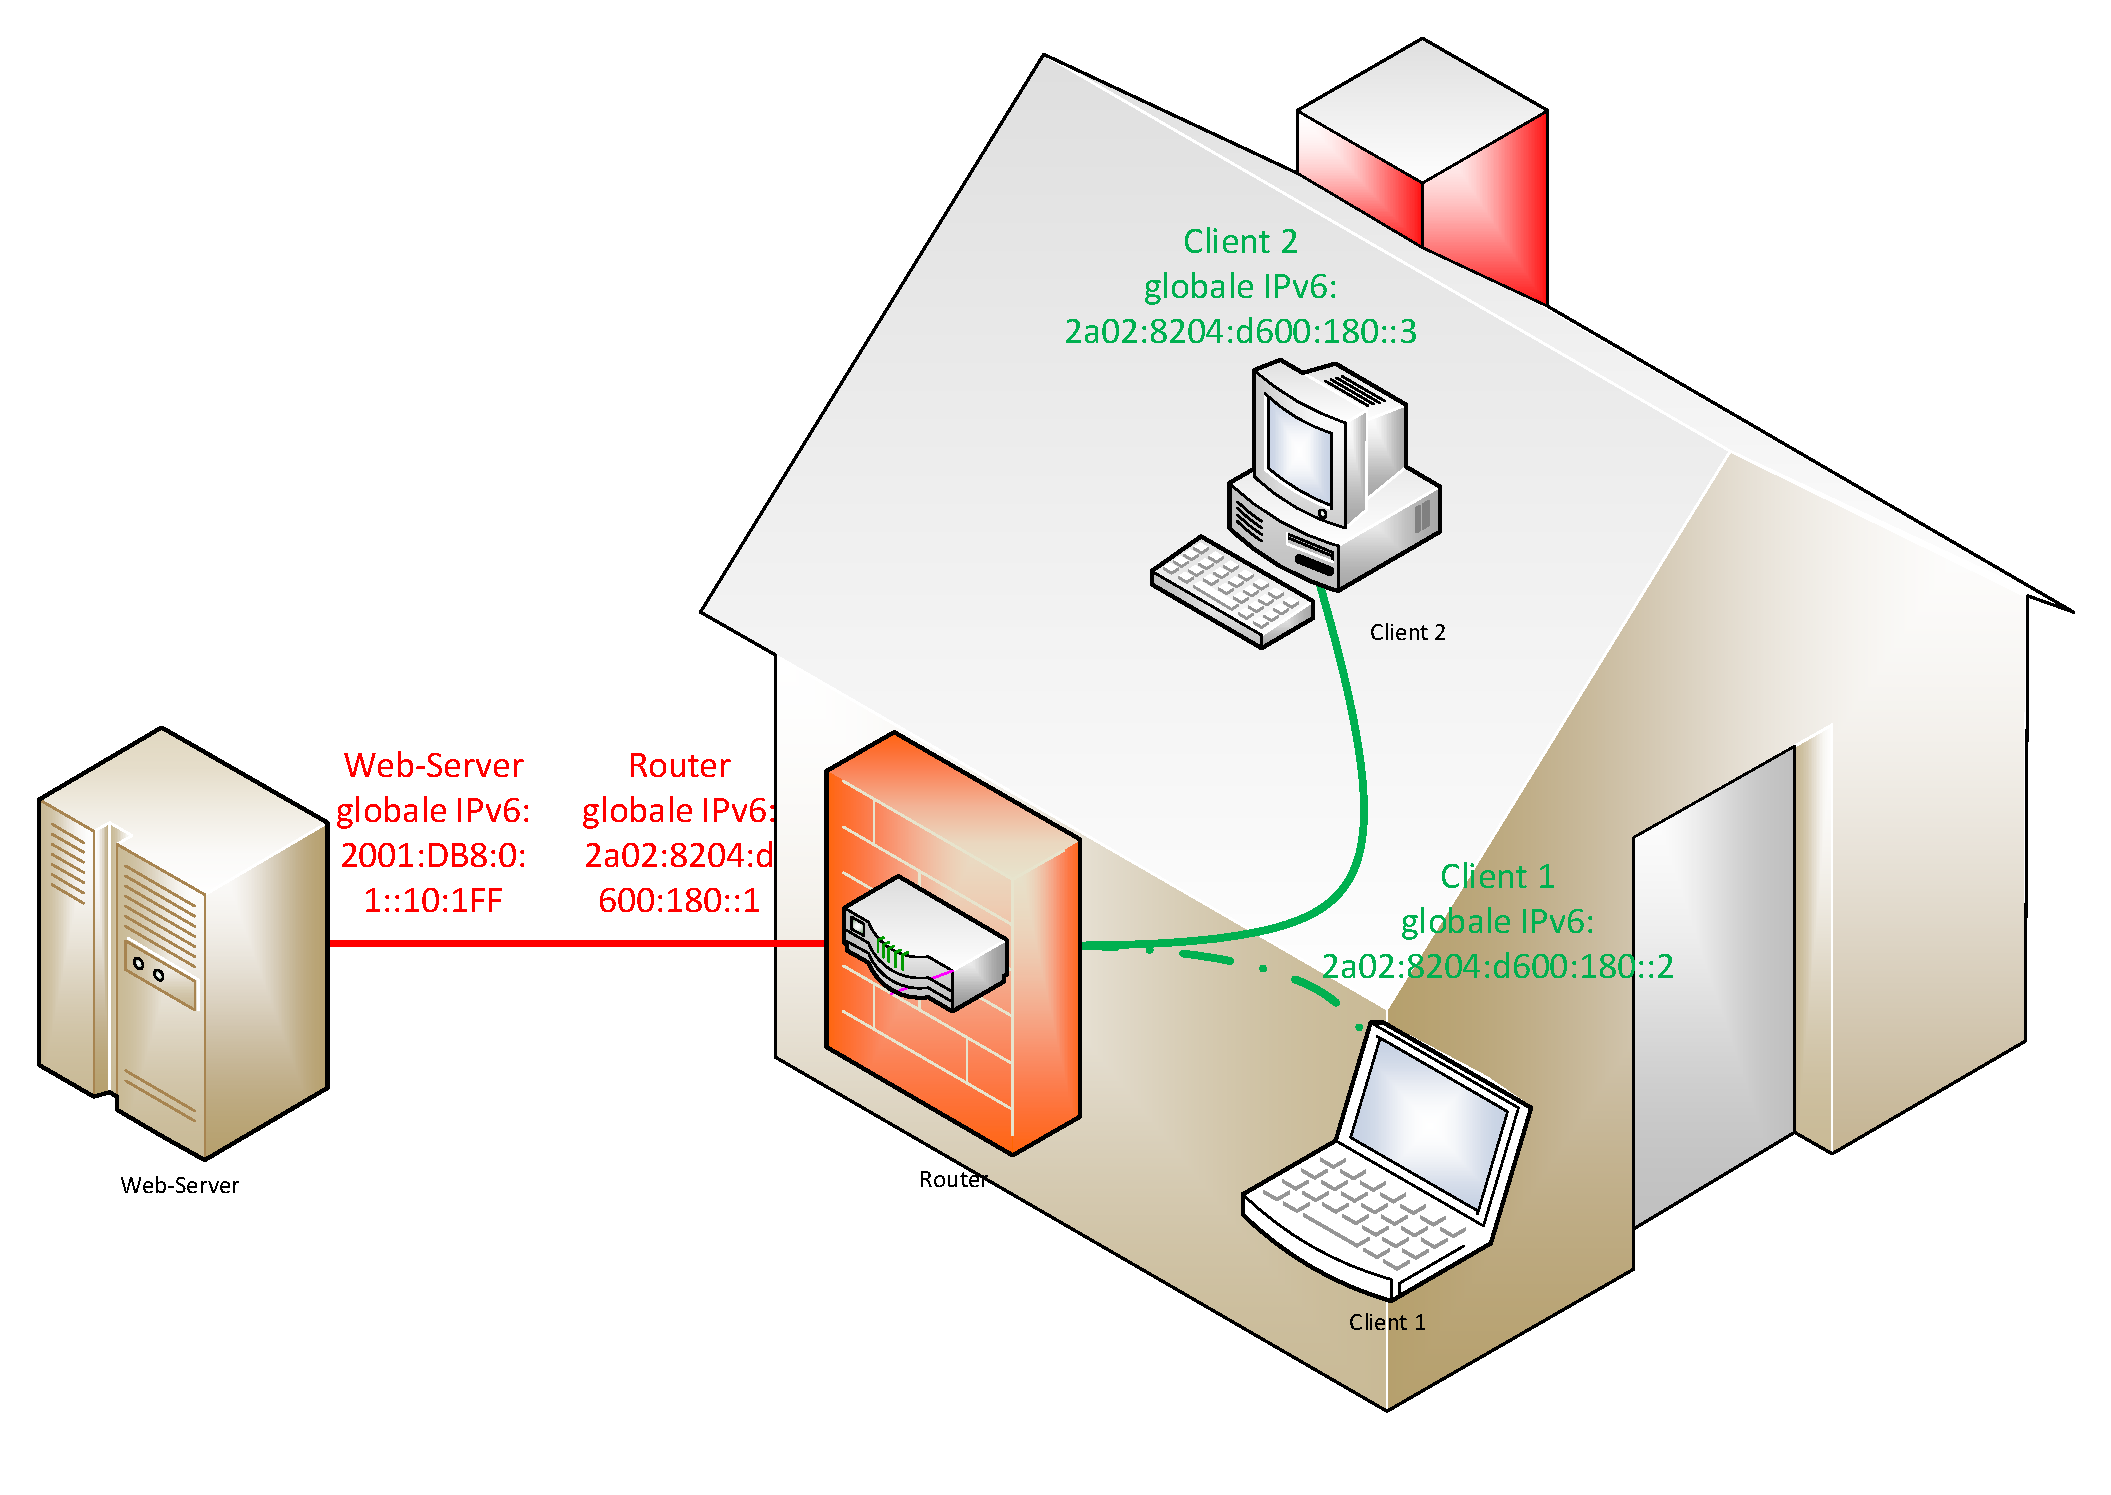
\includegraphics[width=.8\hsize]{./Zeichnungen/IPv6.pdf}
 \end{center}
\caption[Beispielhafte Standardkonfiguration eines Internetanschluss mit nativer IPv6-Konnektivit\"at, Quelle: Autor, verwendete Symbole unterliegen der
GPL]{\label{stdinet}Beispielhafte Standardkonfiguration eines Internetanschluss mit nativer IPv6-Konnektivit\"at.}
\end{figure}

\clearpage
\section{IPv6 heute - Möglichkeiten für Anwender und Administratoren}
Wenn man  Webinhalte \"uber IPv6 abgrufen m\"ochte, ben\"otigt man einen Internetanschluss mit IPv6-Konnektivit\"at. Dazu gibt es zwei M\"oglichkeiten, entweder der verwendete Internet Service Provider stellt IPv6 am Internetnetanschluss direkt zur Verf\"ugung, oder man muss selbst nachbessern. Die beiden M\"oglichkeiten werden im Folgenden n\"aher beschrieben

\subsection{IPv6-Konnektivit\"at nativ vom Internet Service Provider}
Falls der verwendete Internet Service Provider IPv6 nativ am verwendeten Internet Anschlu{\ss} zur Verf\"ugung stellt und auch die eingesetzten Router IPv6-f\"ahig sind, hat der Benutzer nichts weiter zu tun, als sein IPv6-f\"ahiges Netzwerkger\"at mit dem Netzwerk zu verbinden. Durch die in den voran gegangenen Kapiteln vorgestellten, fortschrittlichen Adressfindungsmechanismen in IPv6 wird vollst\"andige Netzwerkkonnektivit\"at ohne manuelles Eingreifen des Benutzers hergestellt.\\
\\
Vom Autor muss an dieser Stelle negativ angemerkt werden, dass zum derzeitigen Zeitpunkt, dass heißt im Jahr 2014, also 15 Jahre nach der finalen Verabschiedung des IPv6-Standards,  keiner der in Deutschland im Privatkundenmarkt t\"atigen Internet Service Provider in der Lage, beziehungsweise Willens ist, dem Kunden IPv6 in nennenswerten Umfang zur Verf\"ugung zu stellen. Entweder wurde noch garnicht mit der Umstellung begonnen, oder der Prozentsatz der Kunden mit nativer IPv6-Konnektivit\"at liegt noch im unterem einstelligen Prozentbereich.\\
\\
Gesch\"aftskunden genie{\ss}en in der Regel den Vorzug einer vielf\"altigen Auswahl im Bezug auf die Internet Service Provider. Es kann daher vom Autor nur angeraten werden, bei der Auswahl der zuk\"unftigen Internet Service Provider die native IPv6-Konnektivt\"at zu einem Schl\"usselkriterium zu machen.

\subsection{IPv6-Konnektivit\"at per Tunnel}
Ist der Anwender an einen Internet Service Provider gebunden, der noch kein natives IPv6 an seinem Internetanschluss zur Verf\"ugung stellt, gibt es noch die M\"oglichkeit mit Hilfe eines IPv6-Tunnels IPv6-Konnektivit\"at zu erm\"oglichen. Es ist bei Anbietern wie \url{https://www.sixxs.net/} m\"oglich, sich kostenfrei einen IPv6-Tunnelendpunk inklusive eines global routbaren 64 Bit gro{\ss}en IPv6-Adressblock zuteilen zu lassen. 

\begin{figure}[htb]
\begin{center}
 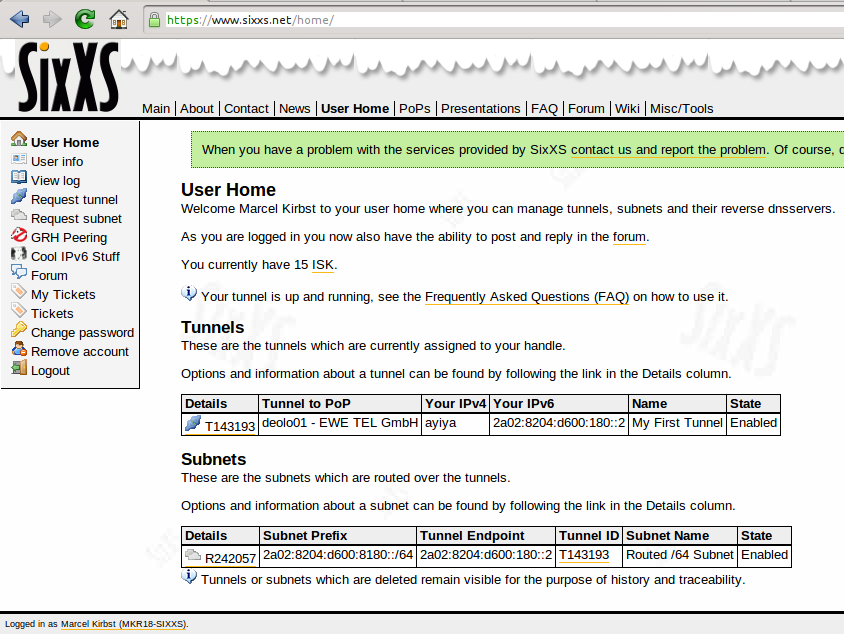
\includegraphics[width=1\hsize]{./images/sixxs.png}
 \end{center}
\caption[Webseite der Anbieters \url{https://sixxs.net} f\"ur einen kostenfreien IPv6-Tunnelendpunkt]{\label{sixxs}Webseite der Anbieters \url{https://sixxs.net} f\"ur einen kostenfreien IPv6-Tunnelendpunkt}
\end{figure}

Ein solcher Tunnel l\"asst sich an einem Router oder auch direkt in einem Netzwerkendger\"at konfigurieren. Setzt man beispielsweise Linux ein, kann man mit dem Softwarepaket \textit{aiccu} sehr einfach die Konfiguration des IPv6-Tunnels vom Typ AYIYA (Anything in Anything, siehe\cite[sixxsayiya]{sixxsayiya} )abschlie{\ss}en. F\"ur das Testsystem mit dem Betriebssystem Kubuntu 12.04 LTS war es nur erforderlich das Paket \textit{aiccu} mittels 

\definecolor{listinggray}{gray}{0.9}
\definecolor{lbcolor}{rgb}{0.9,0.9,0.9}
\lstset{
	language=BASH,
	keywordstyle=\bfseries\ttfamily\color[rgb]{0,0,1},
	identifierstyle=\ttfamily,
	commentstyle=\color[rgb]{0.133,0.545,0.133},
	stringstyle=\ttfamily\color[rgb]{0.627,0.126,0.941},
	showstringspaces=false,
	basicstyle=\scriptsize,
	tabsize=1,
	breaklines=true,	%automatischer Zeilenumbruch
	prebreak = \raisebox{0ex}[0ex][0ex]{\ensuremath{\hookleftarrow}},
	breakatwhitespace=false,
	aboveskip={1.5\baselineskip},
  	columns=fixed,
  	upquote=true,
  	extendedchars=true,
  	backgroundcolor=\color[rgb]{0.97,0.97,0.97},
}
\begin{lstlisting}
$ sudo apt-get install aiccu
\end{lstlisting}

zu installieren und w\"ahrend der Installation die Anmeldedaten zu sixxs.net, dass hei{\ss}t Benutzer und Passwort mitzuteilen. Es werden im Verlauf der Installation dann s\"amtliche Tunnelparameter selbstst\"andig ermittelt und alle Einstellungen so \"ubernommen, dass nach der Installation IPv6-Konnektivität \"uber den Tunnel gew\"ahrleistet ist. Testen l\"asst sich das beispielsweise \"uber die Webseite \url{http://test-ipv6.com/}, die dann folgendes Resultat liefern sollte:

\begin{figure}[htb]
\begin{center}
 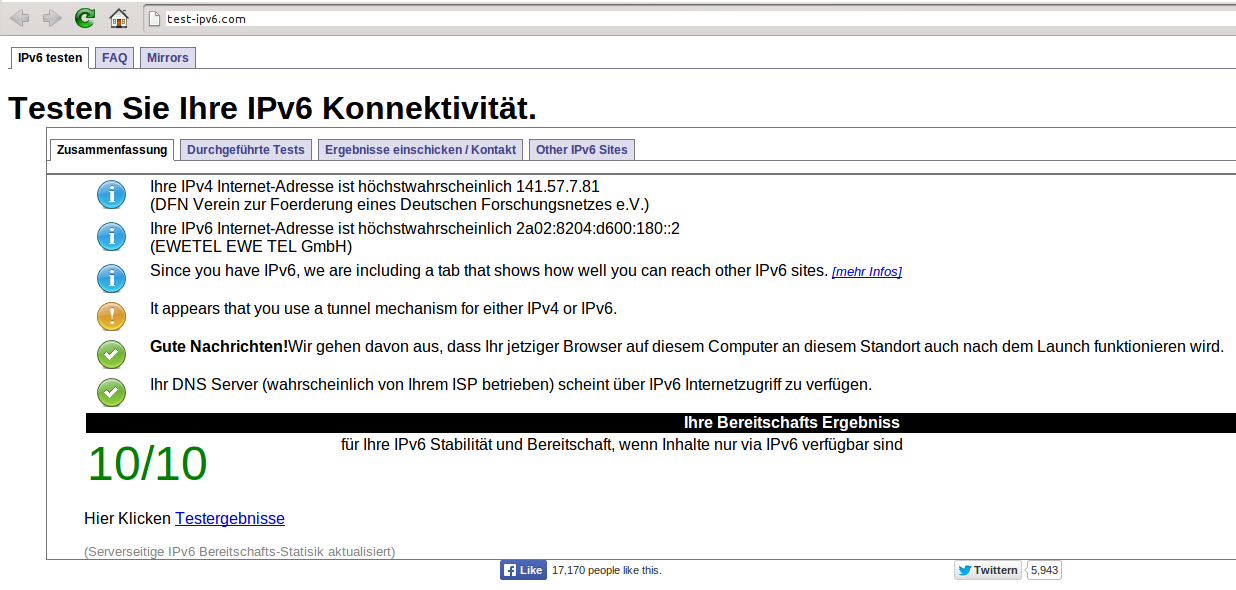
\includegraphics[width=1\hsize]{./images/testipv6.png}
 \end{center}
\caption[Webseite zum Testen der IPv6-Konnektivit\"at: \url{http://test-ipv6.com/}]{\label{testipv6}Webseite zum Testen der IPv6-Konnektivit\"at: \url{http://test-ipv6.com/}}
\end{figure}

%%\clearpage
\section{Zusammenfassung und Ausblick}
Allein durch die immens fortgeschrittene Knappheit an IPv4-Adressen ist ersichtlich, dass der Umstieg zu IPv6 unumg\"anglich ist. Umso schmerzlicher ist im Jahr 2014 festzustellen, wie wenig verbreitet IPv6 noch immer ist. Das gilt f\"ur Internet Service Provider genauso, wie f\"ur Weltkonzerne wie Apple oder IBM, deren Webpräsenzen bis heute nicht über IPv6-Konnektivit\"at verf\"ugen. Es gibt aber auch positive Beispiele, wie beispielsweise der deutsche Hardwarehersteller \url{http://www.avm.de} oder \url{http://www.heise.de}. Es bleibt zu hoffen, dass viele Menschen verstehen, dass IPv6 nicht nur den verf\"ugbaren Adressraum signifikant erh\"oht, sondern auch viele andere technische Unzul\"anglichkeiten ausmerzt, die im Laufe der Jahre bei der Verwendung von IPv4 zu Tage getreten sind. Der Autor ist der Meinung, dass durch hinreichend viele aktive IPv6-Nutzer auch gr\"o{\ss}ere Konzerne, wie auch \"offentliche Einrichtungen\footnote{Die HTWK Leipzig ist im Bezug auf IPv6-Konnektivit\"at leider auch kein positives Beispiel} endlich dazu \"ubergehen, IPv6 nicht mehr so "'stiefm\"utterlich"` zu behandeln, wie es vielerorts bis heute leider der Fall zu sein scheint. 


\clearpage
\section{Literatur- und Quellenverzeichnis}

\renewcommand\refname{Literaturverzeichnis}
\begin{thebibliography}{999}

\bibitem{goncalves1998}Goncalves, Marcus:   {\sl IPv6 Networks} Mcgraw-Hill Professional, 1998,
\\ISBN:  978-0-07024-807-6

\bibitem{dittler2002}Dittler, Hans Peter:  {\sl IPv6 - Das neue Internet-Protokoll, 2. Auflage}. dpunkt-Verlag Heidelberg, 2002,
\\ISBN: 978-3-89864-149-4

\end{thebibliography}

\renewcommand\refname{Quellenverzeichnis}
\begin{thebibliography}{999}

\bibitem{uninet}    
\url{https://www.un.org/Depts/german/menschenrechte/a-hrc-20-L.13.pdf}\\
abrufbar am 03.03.2014

\bibitem{ianaipv4list} \url{https://www.iana.org/assignments/ipv4-address-space/ipv4-address-space.txt}\\
abrufbar am 05.03.2014

\bibitem{RFC1631} RFC1631 - The IP Network Address Translator\\
\url{https://www.ietf.org/RFC/RFC1631.txt}\\
abrufbar am 06.03.2014

\bibitem{RFC2131} RFC2131 - Dynamic Host Configuration Protocol\\
\url{http://tools.ietf.org/html/RFC2131}\\
abrufbar am 05.03.2014

\bibitem{ipv4v6map} \"Ubersichtsgrafik zum Umfang der Routingtabell f\"ur IPv4 und IPv6\\
\url{http://greenbyte.ch/wp-content/uploads/2012/08/ipv4-ipv6.gif?cf3116}\\
abrufbar am 19.03.2014

\bibitem{RFC5156} RFC5156 - Special-Use IPv6 Addresses \\
\url{http://tools.ietf.org/html/RFC5156}\\
abrufbar am 19.03.2014

\bibitem{RFC3122} RFC3122 -  Extensions to IPv6 Neighbor Discovery for Inverse Discovery Specification\\
\url{http://tools.ietf.org/html/RFC5156}\\
abrufbar am 25.03.2014

\bibitem{RFC4861} RFC4861 - Neighbor Discovery for IP version 6 (IPv6) \\
\url{http://tools.ietf.org/html/RFC4861}\\
abrufbar am 25.03.2014

\bibitem{sixxsayiya} AYIYA: Anything In Anything draft-massar-v6ops-ayiya-02\\
\url{http://tools.ietf.org/html/draft-massar-v6ops-ayiya-02}\\
abrufbar am 28.03.2014

\end{thebibliography}
 
 
\end{document}
%-------------------
%Hier endet der Text deiner Hausarbeit
%-------------------